\section*{WRITING TASK 1}
You should spend about 20 minutes on this task.

\begin{quote}\large The diagram illustrates how rainwater is collected and prepared for non-drinking uses in a residential building.
\end{quote}
Describe the main features of the information, select relevant details, and make comparisons where appropriate.

\begin{center}
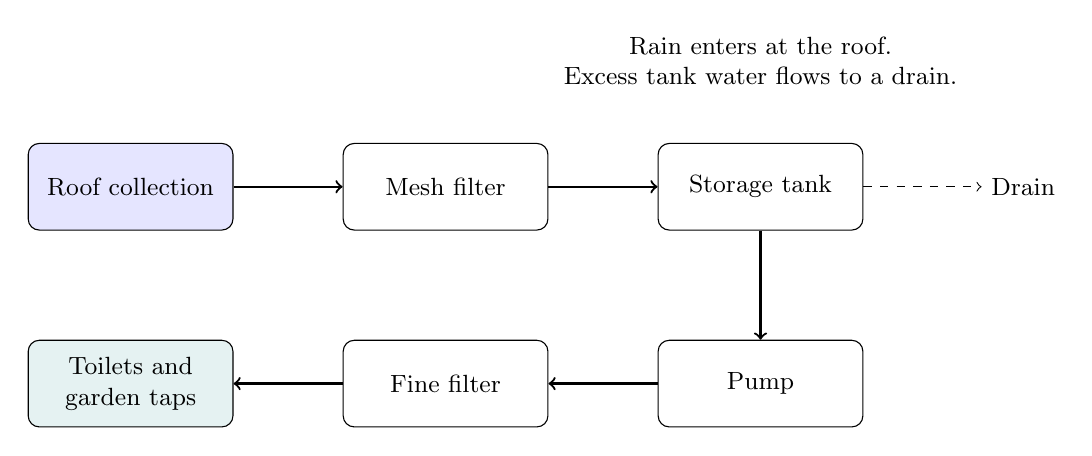
\begin{tikzpicture}[every node/.style={font=\small},box/.style={draw,rounded corners,align=center,minimum width=2.6cm,minimum height=1.1cm}]
\node[box,fill=blue!10] (a) at (0,0){Roof collection};\node[box] (b) at (4,0){Mesh filter};\node[box] (c) at (8,0){Storage tank};
\node[box] (d) at (8,-2.5){Pump};\node[box] (e) at (4,-2.5){Fine filter};\node[box,fill=teal!10] (f) at (0,-2.5){Toilets and\\garden taps};
\draw[->,thick] (a)--(b);\draw[->,thick] (b)--(c);\draw[->,thick] (c)--(d);\draw[->,thick] (d)--(e);\draw[->,thick] (e)--(f);
\node[font=\small,align=center] at (8,1.6){Rain enters at the roof.\\Excess tank water flows to a drain.};\draw[->,dashed] (c.east)--+(1.5,0) node[right]{Drain};
\end{tikzpicture}
\end{center}
Write at least 150 words.
\par\bigskip
{\footnotesize\color{gray} Original practice material; fictional settings and data. Not an official IELTS examination paper.}
